\section{Introduction}
\label{sec:action_actioncategories}

In the last chapter it was shown that a bottom-up method is already powerful enough for complex perception tasks.
A fast moving robot can, without external tracking or external computations, perform safe indoor flights.
However, the robot from the last chapter has no knowledge about higher level symbols like ``door'', ``window'', or ``human being''.
It treats all objects as obstacles alike and performs avoidance maneuvers around them.

The step from symbols to the robot's state space, which is made up of low level motor signals and sensor readings, is called signal-to-symbol gap.
In the next chapter a method is introduced, which will bridge this gap based on a bottom-up method called \glspl{ac:sec}~\cite{aksoy2011learning, aksoydellentamosiunaite2011}.
It generalizes well and it is shown that it allows for complex planning.
The action state space of the flying drone is very limited.
Thus, this chapter deals with a two armed robot: two Kuka Lightweight Robot arms~\cite{bischoff2010kukadlr} mounted on a table as shown in~\figref{fig:sec_introduction_kuka}.
There is one three fingered adaptive robot gripper made by the Schunk company~\cite{schunk2018} attached to each arm.
In this work, only one arm is used since bimanual manipulations are not considered.
As additional sensor input two Asus Xtion Pro cameras~\cite{haggag2013measuring}, one pointing at each arm, and one Nikon D7000 high resolution RGB \gls{ac:dslr} are used.

\begin{figure}
  \centering
  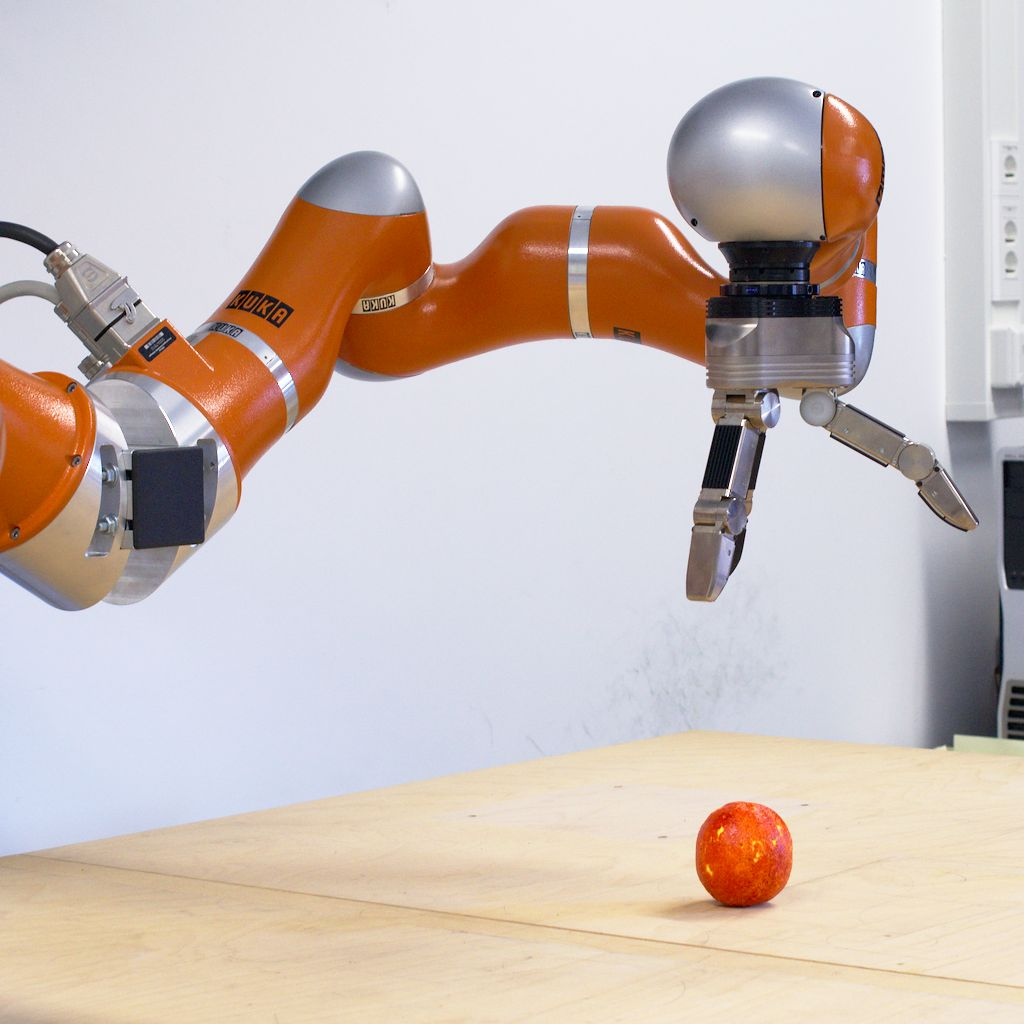
\includegraphics[width=0.5\textwidth]{./figures/sec/kuka.jpg}
  \caption{One of the two Kuka Lightweight Robots~\cite{bischoff2010kukadlr}. Connected to the robot arm is a three-fingered gripper.}
  \label{fig:sec_introduction_kuka}
\end{figure}

In recent years, developments in the field of robotics have emerged solutions to a very wide field of problems: Ranging from autonomous driving to search and rescue missions in remote areas; from space exploration tasks to the care of elderly people.
This also means that robots become more and more integrated into our daily life.
Along come increasingly complex situations, which need to be mastered.
Planning plays a vital part here.

Historically, planning in robotics is divided into two fields: on the one side there are voltages and currents to be controlled.
In this domain physical constraints are most important, \ie robot hardware, collision detection, collision avoidance, and a dynamically feasible trajectory~\cite{choset2005, plaku2010}.
On the other side there are higher level descriptors, which work in the symbolic domain.
One example for two symbols might be \emph{empty cup} and \emph{cup full of water}.
Now, a transfer function \emph{fill cup with water} to arrive at the second symbol from the first can be defined.
Furthermore, the fact that the cup must be empty in order to fill it with water is called precondition.
Preconditions ensure that only transfer functions are applied to symbols, where it makes sense.
For example, filling a full cup with more water would result in spilling.
Similarly, the filled cup is called postcondition of the filling action~\cite[p. 66f., p. 335f.]{golding2006interactive}.
The transition from raw sensor data to a symbolic descriptor is again the above mentioned signal-to-symbol gap and both planning approaches are separated by this gap.
They are considered as two different problems~\cite{arkin1990, payton1990, belta2007}, where the first one is bottom-up and the second one top-down.
In this work, the gap is bridged using a bottom-up method, which requires almost no higher level knowledge.
This is one of the biggest advantages compared to current state-of-the-art.

One of the main obstacles in this field of robotic science is acquiring these symbolic descriptors from sensor data.
This poses a critical problem in two respects.
First, it is needed for logic-based reasoning and the resulting descriptors form the basis for further learning.
Second, it is essential for higher-level planning.
The planning component uses the resulting descriptors instead of sensor data.
There are numerous ways of bridging the signal-to-symbol gap.
First, one needs to define how a logical sequence of sensor signals can be divided into actions and subactions, where each part may be connected to a logical symbol.
Second, this must happen in an automatic manner.

Planning and learning usually happens in the symbolic domain.
A discrete state space, including discrete actions, is assumed.
Throughout the years, a lot of progress has been achieved and various complex domain description languages, such as STRIPS~\cite{fikes1971}, PDDL~\cite{mcdermott1998}, HAL~\cite{marthi2007}, or ADL~\cite{pednault1994}, have been developed to meet the increasingly demanding \gls{ac:ai} tasks.
Various approaches exist to solve discrete problems in the defined domain~\cite{kuter2009} and even high level frameworks exist for easy implementation~\cite{agostinitorraswoergoetter2017, de2009indigolog}.

Thus, more elaborate decision making systems have been proposed to integrate the motion planning more tightly into the action planning domain.
In~\cite{hauser2009, kaelbling2011, plaku2010} a forward-search planner is used.
The task plan is built and the feasibility is continuously checked by a geometric/low level motion planner and being replanned in cases of error.
With this motivation in~\cite{caldiran2009, eyerich2010}, an interface is introduced, which provides ``external predicates''.
These functions are used in the action domain description for checking the feasibility of a primitive action by a motion planner~\cite{erdem2011}.
In~\cite{eyerich2010} the planning language PDDL~\cite{mcdermott1998} is extended with so called semantic attachments and the motion planner is changed accordingly.

It has been shown that there is a fine line when taking low level information, \ie geometric features into account~\cite{erdem2011}.
Obviously, some information is needed for action execution and while a task often can be solved this way, the resulting plan might be inefficient or unfeasible.
Taking some high level information into account, a plan made up from low level information can often be enhanced~\cite{erdem2011}.
In this work, a novel approach to planning on a very low abstraction level is introduced: First, it is shown that even without high level knowledge a very wide variety of tasks on that level can be solved.
Second, this low level of abstraction can be utilized to retrieve a motor signal in a straightforward way, but also can access the higher level symbolic domain easily.
This means, this planner can be used as a way to bridge the signal-to-symbol gap.
Therefore, a third abstraction layer between the motion planner and a high level symbolic planner is employed and thus combines the advantages of low- and high level planning.
Again, actions are represented by Semantic Event Chains.
In this work, it is shown that using \glspl{ac:sec} and further enriching those by pre- and postconditions, an already very powerful action decision framework is built.
This way the framework does not depend on high level symbolic knowledge, but is rather built using a bottom-up method.
